\chapter{Biologia Molecular e Bioinformática}
 
\indent Neste capítulo serão descritos os conceitos básicos da biologia molecular. A seção \ref{acidosNucleicos} ...





%% ================================================================================================================== %%


\section{Ácidos Nucléicos} \label{aceidosNucleicos}

\indent Os ácidos nucléicos são biomoléculas responsáveis pelo armazenamento, transmissão e tradução das informações genéticas dos seres vivos. Isto é possível devido ao processo de síntede de proteínas que permite, assim, a base da herança biológica.Os acidos nucléicos são polímero, macromoléculas formadas por estruturas menores chamadas monômeros, que nesse caso são nucleotídeos. Nucleotídeos são compostos de três elementos: um radical fosfato (HPO$_{4}$), uma pentose, ou seja, um monossacarídeo formado por cinco átomos de carbono, e uma base nitrogenada. Existem cinco tipos de bases nitrogenadas que podem compor um nucleotídeo: Adenina(A), Timina(T), Citosina(C), Guanina(G) e Uracila(U).

\begin{figure}[h]
    \centering
    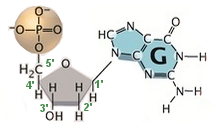
\includegraphics[width=0.4\textwidth]{nucleotideo.png}
    \caption{imagem de um nucleotídeo e das bases nitrogenadas. Mostrar backbone da pentose 1'...5'. Adaptado de : \cite{dnadiscovery08}. }
    \label{fig:Nucleotideo}
\end{figure} 

\indent Na figura \ref{fig:Nucleotideo}, observa-se que no \textit{backbone} do nucleotídeo existe uma numeração de 1' à 5', que representam os carbonos presentes na pentose. Para a criação de uma fita de ácido nucléico, no processo de polimerização fomar-se uma ligação fosfodiéster entre o carbono da posição 5' do \textit{backbone} de um nucleotídeos e o carbono de posição 3' do \textit{backbone} de outro \cite{setubal97}. Por definição o sentido da leitura de uma fita de ácido nucléido é 5' $\rightarrow$ 3', o que é deve ser levado em consideração ao se fazer interpretação de dados do material genético.

\indent Dois tipos de ácidos nucléicos são encontrados nos seres vivos: ácido desoxirribonucleico (DNA) e ácido ribonucleico (RNA). Eles diferenciam-se tanto na estrutura do \textit{backbone} e nas bases nitrogenadas, quanto em suas funções. A seguir serão apresentadas as definições de DNA e RNA.

\subsection{DNA} \label{aceidosNucleicos:dna}

\indent Os DNAs (ou ADN - Ácido Desoxirribonucleico) são as biomoléculas que armazenam as informações referentes ao funcionamento de todas as células dos seres vivos de maneira específica: sequências de pares de bases nitrogenadas. Nesse sentido, além de haver a ligação fosfodiéster entre os nucleotídeos, cada um também se liga a partir de suas bases nitrogenadas, formando assim um eixo helicoidal tridimensional chamada de dupla hélice \cite{setubal97}. Esta estrutura foi descoberta em 1953, pelo biólogo James Watson e pelo físico Francis Crick \cite{dnadiscovery08}, porém os ácidos nucléicos já eram estudado desde 1869 na Suíça pelo químico-fisiológico Friedrich Miescher.

\indent Em relação à estrutura dos monômeros do DNA, o \textit{backbone} dos nucleotídeos é uma desoxirribose, indicada na figura \ref{fig:EstruturasDoDNA}. Para a formação da dupla hélice, os pares são feitos com uma base nitrogenada do grupo de purinas, composto orgânico que possui um anel duplo de carbono, e outra base do grupo de pirimidinas, composto orgânico que possui um anel simples de carbono. No caso do DNA, somente quatro das cinco bases são empregadas: as purinas Adenina(A) e Guanina(G), que se ligam com as pirimidinas Timina(T) e Citosina(C) respectivamente. Desta forma, A e T são bases complementares, assim como G e C. Uma fita de DNA pode conter centenas de milhões de nucleotídeos.

\indent A representação do DNA, seja nos livros ou computacionalmente, é dada por um par em paralelo de strings de letras A, T, G e C. Como explicado no início dessa seção, o sentido padrão da leitura de uma fita é de 5' $\rightarrow$ 3', mas no caso do DNA, as hélices são dispostas de maneira antiparalela, ou seja, uma é lida de 5' $\rightarrow$ 3' e a outra, de 3' $\rightarrow$ 5'. Observa-se que a partir de uma hélice, pode-se inferir a sequência de sua hélice complementar. Seja, por exemplo, uma hélice H1 igual a AGTAAGC; então H2 em seu sentido oposto é H2' igual a TCATTCG, e no sentido regular, igual a GCTTACT. A figura \ref{fig:EstruturasDoDNA} apresenta a estrutura do DNA como explicada nesta seção.

\begin{figure}[h]
    \centering
    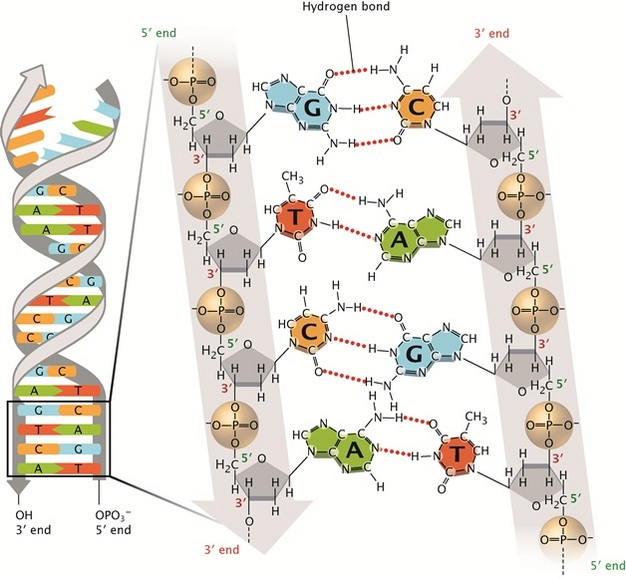
\includegraphics[width=0.7\textwidth]{dnaEstrutura.jpg}
    \caption{Adaptado de : \cite{dnadiscovery08} }
    \label{fig:EstruturasDoDNA}
\end{figure} 


\subsection{RNA} \label{aceidosNucleicos:rna}

\indent Os RNAs são biomoléculas semelhantes ao DNA, porém contam com três diferenças básicas. A primeira é a estrutura do \textit{backbone} dos nucleotídeos, que é composta por uma ribose ao invés de um desoxirribose. A segunda difereça é em relação às bases nitrogenadas, onde a pirimidina Uracila(U) substitui a Timita(T). 
Por fim, o RNA é formado por apenas uma hélice tridimensional.

\indent Existem três tipos de RNAs presentes no citoplasma - espaço entre a membrama plasmática e o núcleo da célula. 
Cada um possui funções específicas que serão detalhadas na seção \textbf{transcricaoTraducaoSintese}. Em suma, O RNA mensageiro (mRNA) é responsável pela transferência de informação do DNA para o RNA ribossômico (rRNA), que por sua vez irá desanexar a proteína do RNA transportador (tRNA) combinando-o com o rRNA, executando assim, a síntese de proteína.



%% ================================================================================================================== %%

\section{Síntese de Proteína} \label{sinteseDeProteina}



\subsection{Proteína} \label{sinteseDeProteina:proteina}

\indent As proteínas são biomoléculas com diversas responsabilidades no corpo dos seres vivos. 
Se fizerem parte do no grupo de proteínas fibrosas, como o colágeno, irão compor a estrutura do corpo e para isso precisam ser resistentes e insolúveis em água. Caso estejam no grupo de proteínas globulares, como a hemoglobina, realizarão processos dinâmico pelo corpo tais como transportações e cataliações \cite{profangela11}.  Cada tarefa é realizada por um proteína com uma estrutura específica e otimizada pra tal.

\indent Assim como os ácidos nucléicos, as proteínas são polímeros, macromoléculas cujos monômeros são aminoácidos. Aminoácidos são moléculas que possuem cinco componentes: amina (NH$_{2}$), carbono (C), hidrogênio (H), ácido carboxílico (COOH) e uma cadeia lateral que funciona como identificador de cada um dos 20 tipos de aminoácidos presentes nos seres vivos. A maneira como eles são criados será explicada com mais detalhes na subseção \ref{sinteseDeProteina:transcricaoTraducaoSintese}, pois envolve um processo complexo de síntese de proteína executado pelo ribossomo. A ligação, ou polimerização, de dois aminoácidos é feita unindo a amida de um com o ácido carboxílico do outro, liberando uma molécula de água (H$_{2}$O) e formando uma cadeia chamada de dipeptídeo. Como houve liberação de água na ligação, o dipeptídeo não é formado por aminoácidos, mas sim resíduos dos mesmos. Nesse sentido, cadeias peptídicas de 100 à 5000 diferentes resíduos aminoácidos, ou cadeia polipeptídicas,  constituem a proteína.

\indent Existem quatro estruturas para caracterização de uma proteína \cite{setubal97}. A mais simples é chamada de estrutura primária e é composta por uma sequência linear de resíduos aminoácidos. A estrutura secundária é tridimensional e estabiliza-se por meio de ligações de hidrogênio na cadeia principal, chamada de \textit{backbone}. Dependendo da disposição dos resíduos de aminoácidos, esta cadeia pode se dar forma de hélice ou em forma de folha. A estrutura terciária é dada pela união de várias estruturas secundárias e, por fim, a estrutura quaternária é composta de múltiplas estruturas terciárias \cite{drug09}. A figura \ref{fig:EstruturasDaProteina} ilustra os quatro tipos de proteínas descritos.

\begin{figure}[h]
    \centering
    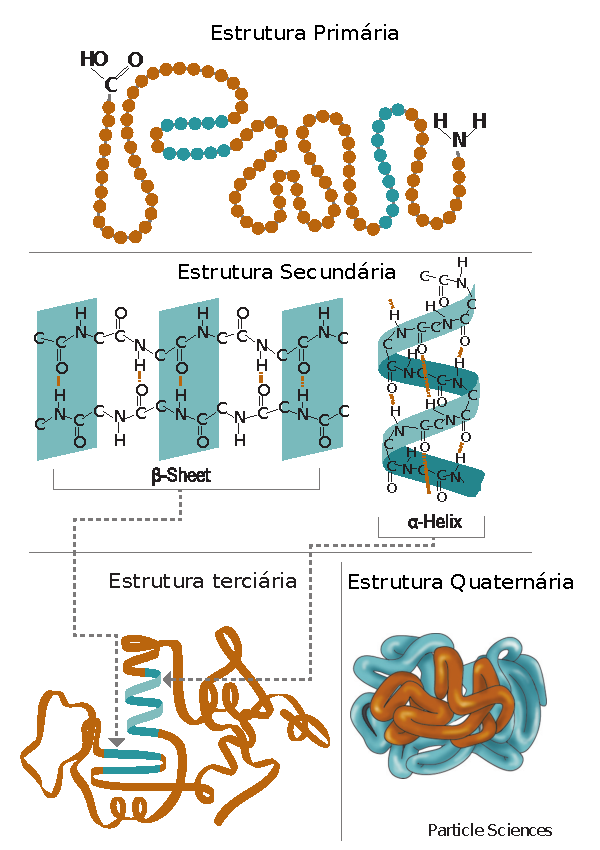
\includegraphics[width=0.5\textwidth]{EstruturasDaProteina.pdf}
    \caption{Adaptado de : \cite{drug09} }
    \label{fig:EstruturasDaProteina}
\end{figure}

\subsection{Código Genético} \label{sinteseDeProteina:codigoGenetico} 

\indent No núcleo de cada célula eucariota, ou no citoplasma das células procariotas, estão localizados as moléculas de DNA, chamadas individualmente por \textbf{cromossomo}. O número de cromossomos em cada célula varia por espécie. No caso dos chimpanzés, o núcleo das células possui 48 cromossomos e no caso dos seres humanos, 46. Note que não existe relação entre o grau evolutivo das espécies e o número de cromossomos nas células. \textbf{EXISTE RELAÇÃO ENTRE DUAS ESPÉCIES COM QUASE A MSM QUANTIDADE DE CROMOSSOMOS, THO??}.

\indent Um cromossomo pode ser representado por vários trechos contíguos de DNA, sendo que cada trecho é chamado de \textbf{gene}. Portanto, pode-se afirmar que o cromossomo é um conjunto (ou lista) de genes. No caso dos seres humanos, cada cromossomo possui de 20 mil à 25 mil genes, e cada gene possui em média 10 mil pares de base. \textbf{BUSCAR A FONTE DISSO. http://www.sobiologia.com.br/conteudos/Corpo/Celula3.php}. Um gene, por sua vez, pode ser representado por vários trechos de três pares de base, sendo que cada trecho é chamado de \textbf{códon}.

\indent Normalmente cada proteína é formada a partir de um gene particular. Mais especificamente, cada aminoácido da proteína é formado a partir de um códon do gene. Entretanto, existem 64 códon possíveis ($4_{ParesDeBase} ^3$) mas somente 20 aminoácidos a serem codificados. Nesse sentido, é comum haver mais de um códon correspondendo à um aminoácio. A tabela \ref{tabelaCodigoGenetico} que apresenta a correspondência entre códons e aminoácios é chamada representa o \textbf{código genético}. \\ \\

\indent CONCLUIR \\


\begin{table}[h!] 
\centering
%\captionsetup{labelsep=space,justification=justified,singlelinecheck=off}
\caption{Código Genético} \label{tabelaCodigoGenetico}
\begin{tabular}{|c|c|c|c|c|c|c|c|}
\hline
 \multirow{2}{*}{ \begin{tabular}[x]{@{}c@{}} Primeira \\ Posição \end{tabular} } & 
 \multicolumn{4}{|c|}{Segunda Posição} & 
 \multirow{2}{*}{ \begin{tabular}[x]{@{}c@{}} Terceira \\ Posição \end{tabular} }\\  \cline{2-5}
 & G & A & C & U &  \\ \hline
 
 \multirow{5}{*}{G} & Gly & Glu & Ala & Val & G \\ 
 					& Gly & Glu & Ala & Val & A \\ 
 					& & & & & 					 \\ 
 					& Gly & Asp & Ala & Val & C \\ 
 					& Gly & Asp & Ala & Val & U \\ \hline 
 					
 \multirow{5}{*}{A} & Arg & Lys & Thr & Met & G \\ 
 					& Arg & Lys & Thr & Ile & A \\ 
 					& & & & & 					 \\ 
 					& Ser & Asn & Thr & Ile & C \\ 
 					& Ser & Asn & Thr & Ile & U \\ \hline 
 					
 \multirow{5}{*}{C} & Arg & Gln & Pro & Leu & G \\ 
 					& Arg & Gln & Pro & Leu & A \\ 
 					& & & & & 					 \\ 
 					& Arg & His & Pro & Leu & C \\ 
 					& Arg & His & Pro & Leu & U \\ \hline 
 					
 \multirow{5}{*}{U} & Trp & \textbf{FIM} & Ser & Leu & G \\ 
 					& \textbf{FIM} & \textbf{FIM} & Ser & Leu & A \\ 
 					& & & & & 					 \\ 
 					& Cys & Asp & Ala & Phe & C \\ 
 					& Cys & Asp & Ala & Phe & U \\ \hline 
 
\end{tabular}
\end{table}




\cite{setubal97}

\subsection{Transcrição e tradução} \label{sinteseDeProteina:transcricaoTraducaoSintese}

\indent rRNA, mRNA, tRNA

\indent síntese de proteína



\section{Bioinformática} \label{bioinformatica}

\subsection{Sequenciamento} 

\indent Mardis 2008

\subsection{Desafio das ômicas}

\indent 
Genômica

\indent Conceitualização do algortimo.

Artigos:
Introdução
[introduction to bioinformatics for computer scientists]